\documentclass{beamer}
%\documentclass[handout]{beamer}
%\usepackage{pgfpages}
%\pgfpagesuselayout{4 on 1}[a4paper,border shrink=5mm,landscape]

% Based on solutions/generic-ornate-15min-45min.en.tex
% and HPCS-UoC-Beamer-master/uoc-beamer-template-1.tex.

% Copyright 2004 by Till Tantau <tantau@users.sourceforge.net>.
%
% In principle, this file can be redistributed and/or modified under
% the terms of the GNU Public License, version 2.
%
% However, this file is supposed to be a template to be modified
% for your own needs. For this reason, if you use this file as a
% template and not specifically distribute it as part of a another
% package/program, I grant the extra permission to freely copy and
% modify this file as you see fit and even to delete this copyright
% notice. 


\mode<presentation>
{
  \usetheme{cambridge}
  %\usetheme{Warsaw}

  \setbeamertemplate{navigation symbols}{}
  \setbeamercovered{transparent}
}

\usepackage[english]{babel}
\usepackage[latin1]{inputenc}
\usepackage{multicol}
\usepackage{hyperref}

\title[HPC: An introduction] % (optional, use only with long paper titles)
{An Introduction to High Performance Computing}

%\subtitle
%{Presentation Subtitle} % (optional)

\author[SJ Rankin, P Sumption, J Salmond] % (optional, use only with lots of authors)
{Stuart Rankin\\ \texttt{support@hpc.cam.ac.uk}}
%{F.~Author\inst{1} \and S.~Another\inst{2}}
% - Use the \inst{?} command only if the authors have different
%   affiliation.

\institute[Research Computing Services, University of Cambridge] % (optional, but mostly needed)
{Research Computing Services (http://www.hpc.cam.ac.uk/ http://www.csd3.cam.ac.uk/)\\
University Information Services (http://www.uis.cam.ac.uk/)}
% - Use the \inst command only if there are several affiliations.
% - Keep it simple, no one is interested in your street address.

\date[18/10/2017] % (optional)
{25th January 2018 / UIS Training}

\subject{Courses}
% This is only inserted into the PDF information catalog. Can be left
% out. 
% If you have a file called "university-logo-filename.xxx", where xxx
% is a graphic format that can be processed by latex or pdflatex,
% resp., then you can add a logo as follows:
% \pgfdeclareimage[height=0.5cm]{university-logo}{university-logo-filename}
% \logo{\pgfuseimage{university-logo}}
% Delete this, if you do not want the table of contents to pop up at
% the beginning of each subsection:
%\AtBeginSubsection[]
%{
%  \begin{frame}<beamer>{Outline}
%    \tableofcontents[currentsection,currentsubsection]
%  \end{frame}
%}

% If you wish to uncover everything in a step-wise fashion, uncomment
% the following command: 

%\beamerdefaultoverlayspecification{<+->}


\begin{document}

\begin{frame}
  \titlepage
\end{frame}

\begin{frame}{Health and Safety}
\begin{columns}[c]
\begin{column}{0.33\textwidth}
\begin{center}

\includegraphics[width=0.8\textwidth,height=0.5\textheight,keepaspectratio]{imgs/health-safety-1.png}\\

\includegraphics[width=0.8\textwidth,height=0.5\textheight,keepaspectratio]{imgs/health-safety-4.png}
\end{center}
\end{column}
\begin{column}{0.33\textwidth}
\begin{center}

\includegraphics[width=0.8\textwidth,height=0.5\textheight,keepaspectratio]{imgs/health-safety-2.png}\\
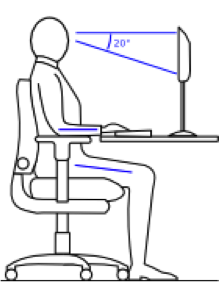
\includegraphics[width=0.8\textwidth,height=0.5\textheight,keepaspectratio]{imgs/health-safety-5.png}
\end{center}
\end{column}
\begin{column}{0.33\textwidth}
\begin{center}

\includegraphics[width=0.8\textwidth,height=0.5\textheight,keepaspectratio]{imgs/health-safety-3.png}\\

\includegraphics[width=0.8\textwidth,height=0.5\textheight,keepaspectratio]{imgs/health-safety-6.png}
\end{center}
\end{column}
\end{columns}
\end{frame}

\begin{frame}<presentation>{Welcome}
\begin{itemize}
\item{Please sign in on the {\color{red}attendance sheet}.}
\item Please fill in the {\color{red}online feedback} at the end of the course:
      \url{http://feedback.training.cam.ac.uk/ucs/form.php}
\item{Keep your belongings with you.}
%\item Course files can be downloaded from:  \url{www.ucs.cam.ac.uk/training/files}
\item\alert{Please ask questions and let us know if you need assistance.}
\end{itemize}
\end{frame}

\begin{frame}<presentation>{Plan of the Course}
\begin{description}
\item[Part 1:]{Introduction}
\item[Part 2:]{Cluster Basics}
\item[Part 3:]{Advanced HPC}
\medskip
\item<2>{\alert{09:30}\hbox to 0pt{\hphantom{{}-15:15}\quad WELCOME\hss}}
\item<2>{\alert{10:00-11:00}\quad Introduction and basics}
\item<2>{\alert{11:00-11:30}\quad Practical and break}
\item<2>{\alert{12:00-12:30}\quad Practical}
\item<2>{\alert{12:30-13:30}\quad LUNCH}
\item<2>{\alert{14:00-14:30}\quad Practical}
\item<2>{\alert{14:45-15:15}\quad Practical}
\item<2>{\alert{15:30-\hbox to 0pt{CLOSE\hss}\hphantom{15:15}}\quad Further discussion}
\end{description}
\end{frame}

\part{Introduction}
\begin{frame}
\partpage
\end{frame}

%\begin{frame}{Basics: Outline}
%\small
%  \tableofcontents[subsectionstyle=hide]%[pausesections]
%\end{frame}

\section{Who are we?}
\begin{frame}{UIS: Research and Institutional Services Division}
Your trainers for today will be:\\
\begin{itemize}
  \item Paul Sumption --- Research Computing Technical Liaison
    \item Simon Flood --- Research Computing System Administrator
  \item Matthew Archer --- Research Software Engineering Team
  \item\alert{Please ask questions and let us know if you need assistance.}
\end{itemize}
\end{frame}

\section{Training Accounts}
\begin{frame}{Basics: Training accounts}
\begin{itemize}
\item{\alert{For our practical exercise's we will use HPC training accounts.}}
\pause
\item{You will find two pieces of paper on your desk.}
\pause
\item{1: A terms and conditions form for you to sign.}
\pause
\item{2: Your training account details.}
\pause
\item{Your training account will only be valid for today.}
\end{itemize}
\end{frame}

\section{Login node for today}
\begin{frame}{Basics: Login node}
\begin{itemize}
\item{\alert{For our practical exercise's we will use the login node: login-cpu.hpc.cam.ac.uk.}}
\pause
\item{Later in the course you will see that different nodes types may require you to use other login nodes.}
\end{itemize}
\end{frame}

\section{Security}
\begin{frame}{Basics: Security}
\begin{itemize}
\item{\alert{Boring but very, very important${}\ldots$}}
\pause
\item{Cambridge IT is under constant attack by would-be intruders.}
\pause
\item{Your data and research career is threatened by intruders.}
\pause
\item{\alert{Cambridge systems} are high profile and popular targets.}
\pause
\item{\alert{Don't let intruders in.}}
\end{itemize}
\end{frame}

\begin{frame}{Basics: Security}
\begin{enumerate}
\item{\alert{Keep your password (or private key passphrase) safe.}}
\pause
\item{\alert{Always choose strong passwords.}}
\pause
\item{\alert{Your UIS password is used for multiple systems so keep it secure!}}
\pause
\item{Keep the software on your laptops/tablets/PCs up to date this includes home computers especially if you are using the VPN to connect in.}
\pause
\item{Don't share accounts (this is against the rules anyway).}
\end{enumerate}
\end{frame}

\section{Basics: Pre-requisites}
\begin{frame}{Pre-requisites}
\begin{itemize}
\item{A pre-requisite of this course:}
\pause
\item{Basic Unix/Linux command line experience}
\item{\url{https://www.training.cam.ac.uk/ucs/Course/ucs-unixintro1} Unix: Introduction to the Command Line Interface (Self-paced)}
\pause
\item{Shell scripting experience is desirable}
\item{\url{https://www.training.cam.ac.uk/ucs/Course/ucs-scriptsci} Unix: Simple Shell Scripting for Scientists}
\end{itemize}
\end{frame}

\subsection{Navigating the command line }
\begin{frame}{Navigating your terminal}
Useful commands for navigating your terminal.
\begin{itemize}
\item{\alert{\footnotesize cd \textless dirname \textgreater } - change into a directory }
\item{\alert{\footnotesize ls \textless dirname \textgreater } - list the contents of a directory}
\item{\alert{\footnotesize cd or cd \path{~}} - change into your home folder}
\item{\alert{\footnotesize cd .. } - change back one folder}
\item{\alert{\footnotesize man ls } - will bring up the manual page for the ls command}
\item{\alert{\footnotesize pwd } - print working directory}
\end{itemize}
\end{frame}

\part{HPC Basics}
\frame{\partpage}

\begin{frame}{HPC Basics: Our Clusters}
\begin{itemize}
\item{Our clusters are built using lots of commodity servers which then operate as a 'super computer'.}
\pause
\item{We have CPU and GPU cluster nodes.}
\pause
\item{A cluster has a scheduler which runs jobs from a queue.}
\pause
\item{You submit jobs to the queue using a submission script.}
\pause
\item{Jobs have service levels and QOS (quality of service) associated with them.}
\pause
\item{There is a user environment this allows you to load or unload versions of software.}
\pause
\item{We will look at each of these aspects in more detail during the course.}
\end{itemize}
\end{frame}

\section{Why use an HPC cluster?}
\begin{frame}{HPC Basics: Why use an HPC cluster?}
There are many reasons why you may need to use a big computer or cluster. 
\begin{description}
\pause
\item[\textit{Limited local resources:}]{Your jobs can no longer run on your own computer or run very slowly.}
\pause
\item[\textit{Storage Intensive:}]{Your data will exceed that of your local storage capacity.}
\pause
\item[\textit{Software:}]{Many of the software packages you require have a complex installation process or require specialist support.}
\pause
\item[\textit{Grants and sharing:}]{You want to make the best use of your grant when buying computing resources or need to share data or a workflow with your group.}
\end{description}
\end{frame}

\section{Types of job}
\begin{frame}{HPC Basics: Types of problem part 1.}
In this section we will cover high throughput and compute intensive jobs. We will  introduce the user and module environment and submit some High Throughput jobs to some CPU nodes.
\begin{description}
\pause
\item[\textit{High Throughput:}]{Many unrelated problems to be executed in bulk.}
\pause
\item[\textit{Compute Intensive:}]{A single problem requiring a large amount of computation.}
\end{description}
\end{frame}

\subsection{High Throughput}
\begin{frame}{HPC Basics: High Throughput}
\begin{itemize}
\item{Distribute \alert{independent}, \alert{multiple problems} across multiple CPUs to reduce the overall execution time.}
\pause
\item{Workload is trivially (or \emph{embarrassingly}) parallel:}
\begin{itemize}
\item[$\ast$]{Workload breaks up naturally into \emph{independent} pieces.}
\item[$\ast$]{Each piece is performed by a separate process/thread on a separate CPU (concurrently).}
\item[$\ast$]{\alert{Little or no inter-CPU communication}.}
\end{itemize}
\pause
\item{Emphasis is on throughput over a period, rather than on performance on a single problem.}
\pause
%\item{Compute intensive capable $\Rightarrow$ high throughput capable}
%\pause
%\item{\color{red}Compute intensive capable $\not\Leftarrow$ high throughput capable} 
\end{itemize}
\end{frame}

\subsection{Data Intensive}
\begin{frame}{HPC Basics: Data Intensive Problems}
\begin{itemize}
\item{Distribute the \alert{data} for a \alert{single problem} across multiple CPUs to reduce the overall execution time.}
\pause
\item{The \emph{same} work may be done on each data segment.}
\pause
\item{Rapid movement of data to and from disk is more important than inter-CPU communication.}
\pause
\item{\alert{Big Data} problems of great current interest -}
\item{Hadoop/MapReduce}
\item{Life Sciences (genomics) and elsewhere.}
\end{itemize}
\end{frame}

\subsection*{Summary}
\begin{frame}{HPC Basics: Summary}
  \begin{itemize}
  \item<1->{\alert{Why have a supercomputer?}}
  \begin{itemize}\item<2->{Big single problems, many problems, Big Data.}\end{itemize}
  \item<3->{Most current supercomputers are \alert{clusters} of separate \alert{nodes}.}
  \end{itemize}
  
\end{frame}

\section{User Environment Introduction}
\begin{frame}{HPC Basics: User Environment}
\begin{itemize}
\item{The user environment can be changed by loading modules.}
\item{At login some default modules are loaded.}
\item{When you start to compile software or write your own programs you will need to know more about your user environment and the underlying hardware.}
\end{itemize}
\end{frame}

\section{User Environment}
\begin{frame}{HPC Basics: User Environment}
\begin{itemize}
\item<1,4>{\visible<1>{Scientific Linux 6.8 (}\alert<1>{{\color<4>{red}Red Hat Enterprise Linux 6}\visible<1>{.8 rebuild)}}}
\begin{itemize}
\item{\visible<1>{bash}}
\item{\visible<1>{GNOME2 or XFCE4 desktop \alert{(if you want)}}}
\end{itemize}
%\item<1,4>{\visible<1>{Lustre 2.4.1 (patched), Mellanox OFED 3.3,} {\color<4>{red}CUDA 8}\visible<1>{.0}}
\item<1,4>{\visible<1>{Lustre (patched), Mellanox OFED, CUDA}}
\item<2->{But you don't need to know that. \visible<3->{\alert{(Probably\ldots)}}}
\item<5->{Upgrade to Scientific Linux/Red Hat Enterprise Linux 7 underway (Wilkes and new CSD 3 nodes are already on SL7).}
\end{itemize}
\end{frame}

\subsection{Filesystems}
\begin{frame}{User Environment: Filesystems}
When you apply for an HPC account a home directory is created for you. 
\begin{itemize}
\item{\alert{/home/abc123}}
\begin{itemize}
\item{40GB quota.}
\item{Visible equally from all nodes.}
\item{Single storage server.}
\item{Hourly, daily, weekly snapshots copied to tape.}
\item{Not intended for job outputs or large/many input files.}
\end{itemize}
\item{\alert{/scratch/abc123}}
\begin{itemize}
\item{Visible equally from all nodes.}
\item{Larger and faster (1TB initial quota).}
\item{Intended for job inputs and outputs.}
\item{{\color{red}Not backed up.}}
 \pause
\end{itemize}
\end{itemize}
\end{frame}

\subsection{Exceeding 1TB of scratch}
\begin{frame}{Our storage services}
\begin{itemize}
\item{We have several storage services for users that need to exceed 1TB.}
\pause
\item{\alert{http://www.uis.cam.ac.uk/initiatives/storage-strategy/storage-services}}
\item{The most relevant services to HPC are RCS and RDS.}
\item{RCS - Research Cold Store is for data that isn't changing, data goes to disk then two sets of tapes.}
\item{RDS - Research Data Store, non backed up high performance storage for projects.}
\end{itemize}
\end{frame}

\begin{frame}[fragile]{Filesystems: Quotas}
\begin{itemize}
\item{quota}
\begin{semiverbatim}
\tiny
====================================================================================
Usage on /scratch (lfs quota -u abc123 /scratch):
====================================================================================
Disk quotas for user abc123 (uid 456):
      Filesystem  kbytes   quota   limit   grace   files   quota   limit   grace
 /scratch/abc123 \only<1|handout:1>{9298708}\only<2-|handout:2->{{\color{red}*1073742000}}  1073741824 1181116006   -   165588       0       0       -
...
\end{semiverbatim}
\item<1-|handout:1->{\alert{Aim to stay below the soft limit (\emph{quota}).}}
\item<2-|handout:1->{\alert{Once over the soft limit, you have 7 days grace to return below.}}
\item<3-|handout:2>{\alert{When the grace period expires, or you reach the hard limit (\emph{limit}), no more data can be written.}}
\item<4-|handout:2>{\alert{It is important to rectify an out of quota condition ASAP.}}
\end{itemize}
\end{frame}

\begin{frame}{Filesystems: Backups}
\begin{itemize}
\item<1->{Disk snapshots and tape (as of May 2017).}
\item<2->{{\color{red}They are not an undelete - take care when deleting.}}
\item<3->{Successful restoration depends on:}
\begin{itemize}
\item{The file having existed long enough to have been backed up at all.}
\item{The last good version existing in a current backup.}
\item<4->{\color{red}Request restoration as soon as possible with \emph{location} and \emph{exact time of loss}.}
\medskip
\visible<5->{\item{\color{purple}\huge Scratch files are not backed up.}}
\end{itemize}
\end{itemize}
\end{frame}

\begin{frame}{Filesystems: Automounter}
\begin{itemize}
\item{Directories under /scratch are \alert{automounted}.}
\item{They only appear under /scratch when explicitly referenced.}
\item{Thus when browsing /scratch may appear too empty\hfill\\
\qquad\alert{--- use \emph{ls} or \emph{cd} to reference /scratch/abc123 explicitly.}}
\end{itemize}
\end{frame}

\begin{frame}{Filesystems: Permissions}
\begin{itemize}
\item{\color{red}Be careful and if unsure, please ask support@hpc.cam.ac.uk.}
\begin{itemize}
\item{Can lead to \alert{accidental destruction} of your data or \alert{account compromise}.}
\end{itemize}
\item{Avoid changing the permissions on your home directory.}
\begin{itemize}
\item{Files under /home are particularly security sensitive.}
\item{Easy to break passwordless communication between nodes.}
\end{itemize}
\end{itemize}
\end{frame}

\section{Software}
\begin{frame}{Using HPC: Software}
\begin{itemize}
\item{Free software accompanying \alert{Red Hat Enterprise} is (or can be) provided.}
\item{Other software (free and non-free) is available via \alert{modules}.}
\item{Some proprietary software may not be generally accessible.}
\item{See \alert{http://www.hpc.cam.ac.uk/using-clusters/software}.}
\item{New software may be possible to provide on request.}
\item{\alert{Self-installed software must be properly licensed.}}
  \pause
\item{\color{red}\emph{sudo will not work.}\/ (You should be worried if it did.)}
\end{itemize}
\end{frame}

\subsection{Environment Modules Pt 1}
\begin{frame}[fragile]{User Environment: Environment Modules}
\begin{itemize}
\item{Modules load or unload additional software packages.}
\item{Some are \alert{required} and automatically loaded on login.}
\item{Others are optional extras, or possible replacements for other modules.}
\item{\alert{Beware} unloading default modules in $\tilde{}\text{/.bashrc}$.}
\item{\alert{Beware} overwriting environment variables such as PATH and LD\_LIBRARY\_PATH in $\tilde{}\text{/.bashrc}$. If necessary append or prepend.}
\end{itemize}
\end{frame}

\subsection{Environment Modules Pt 2}
\begin{frame}[fragile]{User Environment: Environment Modules}
\begin{itemize}
\item{Currently loaded:}
\begin{semiverbatim}
\scriptsize
module list
Currently Loaded Modulefiles:
  1) dot                     6) intel/impi/4.1.3.045   11) default-impi
  2) scheduler               7) global                 
  3) java/jdk1.7.0_60        8) intel/cce/12.1.10.319  
  4) turbovnc/1.1            9) intel/fce/12.1.10.319  
  5) vgl/2.3.1/64           10) intel/mkl/10.3.10.319
\end{semiverbatim}
\medskip
\item{Available:}
\begin{semiverbatim}
\scriptsize
module av
\end{semiverbatim}
\end{itemize}
\end{frame}

\begin{frame}[fragile]{User Environment: Environment Modules}
\begin{itemize}
\item{Show:}
\begin{semiverbatim}
\tiny
module show castep/impi/7.0.3
-------------------------------------------------------------------
/usr/local/Cluster-Config/modulefiles/castep/impi/7.0.3:

module-whatis    adds CASTEP 7.0.3 (Intel MPI) to your environment 

Note that this software is restricted to registered users.

prepend-path     PATH /usr/local/Cluster-Apps/castep/impi/7.0.3/bin:/usr/local/...
-------------------------------------------------------------------
\end{semiverbatim}
\medskip
\item{Load:}
\begin{semiverbatim}
\scriptsize
module load castep/impi/7.0.3
\end{semiverbatim}
\medskip
\item{Unload:}
\begin{semiverbatim}
\scriptsize
module unload castep/impi/7.0.3
\end{semiverbatim}
\end{itemize}
\end{frame}

\begin{frame}[fragile]{User Environment: Environment Modules}
\begin{itemize}
\item{Matlab}
\begin{semiverbatim}
\scriptsize
module load matlab/r2015b
\end{semiverbatim}
\medskip\pause
\item{Invoking matlab in batch mode:\hfill\\
  \qquad \alert{matlab -nodisplay -nojvm -nosplash command}\hfill\\
  where the file \alert{command.m} contains your matlab code.}
  \pause
  \item{The University site license contains the Parallel Computing Toolbox.}
\end{itemize}
\end{frame}

\begin{frame}[fragile]{User Environment: Environment Modules}
\begin{itemize}
\item{Purge:}
\begin{semiverbatim}
\scriptsize
module purge
\end{semiverbatim}
\smallskip
\item{Defaults:}
\begin{semiverbatim}
\scriptsize
module show default-impi
module unload default-impi
module load default-impi-LATEST
\end{semiverbatim}
\medskip
\item{If you have compiled software yourself your run time environment must match compile time environment!}
\end{itemize}
\end{frame}

\subsection{Modules: Excercise 4}
\begin{frame}[fragile]{Excercise 4: Environment Modules}
\begin{itemize}
\item{Connect to the cluster using your training account: See excercise 2 if you have closed your terminal. }
\item{Get a list of modules that are currently loaded}
\item[\emph{Hints:}]{\alert{module list}}
\item{Get a list of available R modules}
\item[\emph{Hints:}]{\alert{module av R}}
\end{itemize}
\end{frame}

\subsection{Modules: Excercise 5}
\begin{frame}[fragile]{Excercise 5: Run an Rscript}
\begin{itemize}
\item{Connect to the cluster using your training account: See excercise 2 if you have closed your terminal. }
\item{In the exercises folder there is a file called test.r}
\item{Run this script using: Rscript hello.r }
\item{Load the module for: R/3.3.2}
\item[\emph{Hints:}]{\alert{module load R/3.3.2}}
\item{Run the script again: Rscript hello.r}
\end{itemize}
\end{frame}

\section{Storage}
\begin{frame}{HPCS: Storage}
\begin{itemize}
\item{Multi-petabytes split across multiple filesystems with tape.}
\item{Lustre cluster filesystem:}
\begin{itemize}
\item[$\ast$]{Multiple RAID6 back-end disk volumes.}
\item[$\ast$]{Multiple object storage servers.}
\item[$\ast$]{Single metadata server.}
\item[$\ast$]{Tape-backed HSM on newest filesystems.}
\pause
\item[$\ast$]{\alert{$4\,\text{GB/sec}$ overall read or write.}}
\pause
\item[$\ast$]{\alert{Prefers big read/writes over small.}}
\end{itemize}
\pause
\item{\alert{For active HPC work only.}}
\end{itemize}
\end{frame}

\section{Service Levels}
\begin{frame}{HPCS: Service Levels}
\begin{description}
\visible<1-4>{\item[\textbf{Service Level 1}]{Paying, intended for large projects with long-term, consistent requirement.}}
\begin{itemize}
\visible<2-4>{\item{\alert{Guaranteed fraction of resources per quarter.}}}
\end{itemize}
\visible<1-5>{\item[\textbf{Service Level 2}]{Paying, intended for medium-sized projects with irregular requirement.}}
\begin{itemize}
\visible<3-5>{\item{\alert{High priority, but no guarantees; \emph{ad hoc}.}}}
\end{itemize}
\visible<1-4>{\item[\textbf{Service Level 3}]{Non-paying, intended for interim or pump priming, small-scale use.}}
\begin{itemize}
\visible<4>{\item{\alert{Low priority, limited usage (200,000 Darwin core hours) per quarter.}}}
\end{itemize}
\end{description}
\end{frame}

\begin{frame}{HPCS: Service Levels}
\begin{description}
\item[\textbf{Service Level 4}]{Non-paying, for when nothing else is available.}
\pause
\item{\alert{Very low priority, very restricted, very limited. Best efforts continuation.}}
\end{description}
\end{frame}

\section{How To Apply}
\begin{frame}{HPCS: How To Apply}
\begin{itemize}
\item{Submit the online application form:\hfill\\
\qquad\alert{\tiny https://www.hpc.cam.ac.uk/services/applying-for-resources/hpc-application}}
\item{The PI should be someone senior enough to have funding.\hfill\\
\qquad E.g.\ \alert{supervisor}, \alert{head of research group}.}
\pause
\item{\color{red}Funding is not necessary.}
\pause
\item{Please email \alert{support@hpc.cam.ac.uk} for all support issues.}
\item{Further information can be found on the web site:\hfill\\
  \qquad \alert{http://www.hpc.cam.ac.uk}}
  \pause
  \item{\alert{Imminent upgrades may introduce changes.}}
\end{itemize}
\end{frame}

\part{Using HPC}
\frame{\partpage}





\part{Advanced HPC}

\section{Types of job part 2}
\begin{frame}{Advanced HPC: Types of problem.}
In this section we will cover Memory Intensive and Data Intensive jobs.
\begin{description}
\item[\textit{Memory Intensive:}]{A single problem requiring a large amount of memory.}
\pause
\item[\textit{Data Intensive:}]{A single problem operating on a large amount of data.}
\end{description}
\end{frame}

\subsection{Compute Intensive}
\begin{frame}{Advanced: Compute Intensive Problems}
\begin{itemize}
\item{Distribute the \alert{work} for a \alert{single problem} across multiple CPUs to reduce the execution time as far as possible.}
\pause
\item{Program workload must be \emph{parallelised}:}
\begin{description}
\item{Parallel programs split into copies (processes or threads).}
\item{Each process/thread performs a part of the work on its own CPU, concurrently with the others.}
\item{A well-parallelised program will fully exercise as many CPUs as there are processes/threads.}
\end{description}
\pause
\item{The CPUs typically need to exchange information rapidly, requiring specialized communication hardware.}
\pause
\item{Many use cases from Physics, Chemistry, Engineering, Astronomy, Biology...}
\item{The traditional domain of \alert{HPC} and the \alert{Supercomputer}.}
\end{itemize}
\end{frame}

\subsection{Amdahls law pt 1}
\begin{frame}{Advanced: Scaling \& Amdahl's Law}
\begin{itemize}
\item{\alert{Using more CPUs is not necessarily faster.}}
  \pause
\item{Typically parallel codes have a \alert{scaling limit}.}
\item{Partly due to the system overhead of managing more copies, but also to more basic constraints;}
\pause
\item{Amdahl's Law (idealized):}
\[
S(N)=\frac{1}{\left(1-p+\frac{p}{N}\right)}
\]
where \begin{align*}S(N)&\text{ is the fraction by which the program has sped up}\\&\text{ relative to $N=1$}\\
p&\text{ is the fraction of the program which can be parallelized}\\
N&\text{ is the number of CPUs.}
\end{align*}
\end{itemize}
\end{frame}

\subsection{Amdahls law pt 2}
\begin{frame}{Advanced: Amdahl's Law}
\centerline{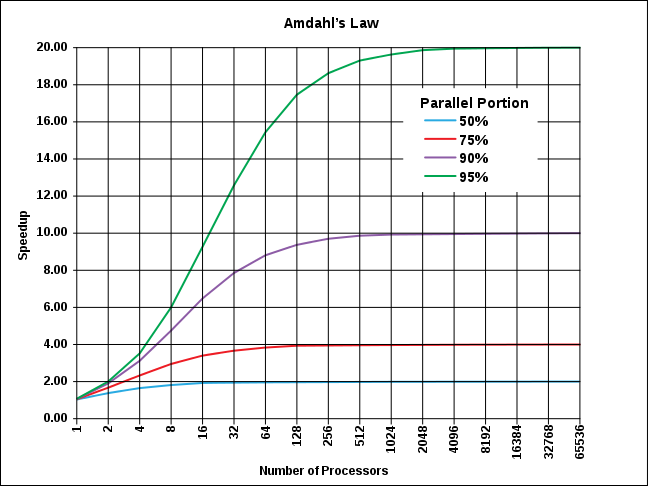
\includegraphics[width=0.75\textwidth]{imgs/AmdahlsLaw.png}}%
\rightline{\tiny http://en.wikipedia.org/wiki/File:AmdahlsLaw.svg}
\smallskip
\end{frame}

\subsection{Compute Intensive Summary}
\begin{frame}{Summary}
\begin{itemize}
\item{Parallelisation requires effort:}
\begin{itemize}
\item{There are libraries to help (e.g. \alert{OpenMP}, \alert{MPI}).}
\item{First optimise performance on one CPU, then make $p$ as large as possible.}
\end{itemize}
\pause
\item{The scaling limit: eventually using more CPUs becomes \alert{detrimental} instead of helpful.}
\end{itemize}
\end{frame}

\subsection{Memory Intensive}
\begin{frame}{Advanced HPC: Memory Intensive Problems}
\begin{itemize}
\item{Require aggregation of large memory rather than multiple CPUs.}
\pause
\begin{description}
\item{\alert{NB Memory (fast, volatile) vs disk (slow, non-volatile).}}
\end{description}
\pause
\item{Technically more challenging to build machines (interconnecting memory \alert{and} CPUs).}
\pause
\item{Coding/porting easier (memory appears seamless, allowing a \alert{single system image}).}
\pause
\item{Optimisation harder (nonuniform memory produces latency).}
\pause
\item{Historically, the arena of large \alert{SGI} systems.}
\pause
\item{Nowadays, similar techniques are applicable to commodity servers.}
\end{itemize}
\end{frame}

\section{architecture}
\begin{frame}{Advanced HPC: Architecture}
\begin{itemize}
\item{So far we have abstracted you from the architecture and the concept of compiling code.}
\item{When does the underlying archictecture start to become important?}
\item{When you are compiling code}
\item{working with MPI/OpenMP}
\item{large job optimisation}
\end{itemize}
\end{frame}

\subsection{Inside a Modern Computer}
\begin{frame}{Advanced HPC: Inside a Modern Computer}{CPUs in a box}
\begin{itemize}
\item<2->{Today's commodity servers already aggregate both CPUs and memory.}
\item<3->{Even small computers now have multiple CPU cores per socket\hfill\\
\visible<4->{\alert{$\implies{}$each socket is a Symmetric Multi-Processor (SMP).}}}
\item<5->{Larger computers have multiple sockets (each with local memory):\hfill\\
{}\qquad all CPU cores (unequally) share the node memory\hfill\\
{}\qquad \visible<6->{$\implies{}$the node is a \alert{shared memory} multiprocessor}\\
{}\qquad \visible<7->{with Non-Uniform Memory Architecture (\alert{NUMA})}\\
{}\qquad \visible<8->{but users still see a single computer (\alert{single system image}).}}
\end{itemize}
\end{frame}

\subsection{Inside a Modern Computer}
\begin{frame}{Advanced HPC: Inside a Modern Computer}{CPUs in a box}
{\centerline{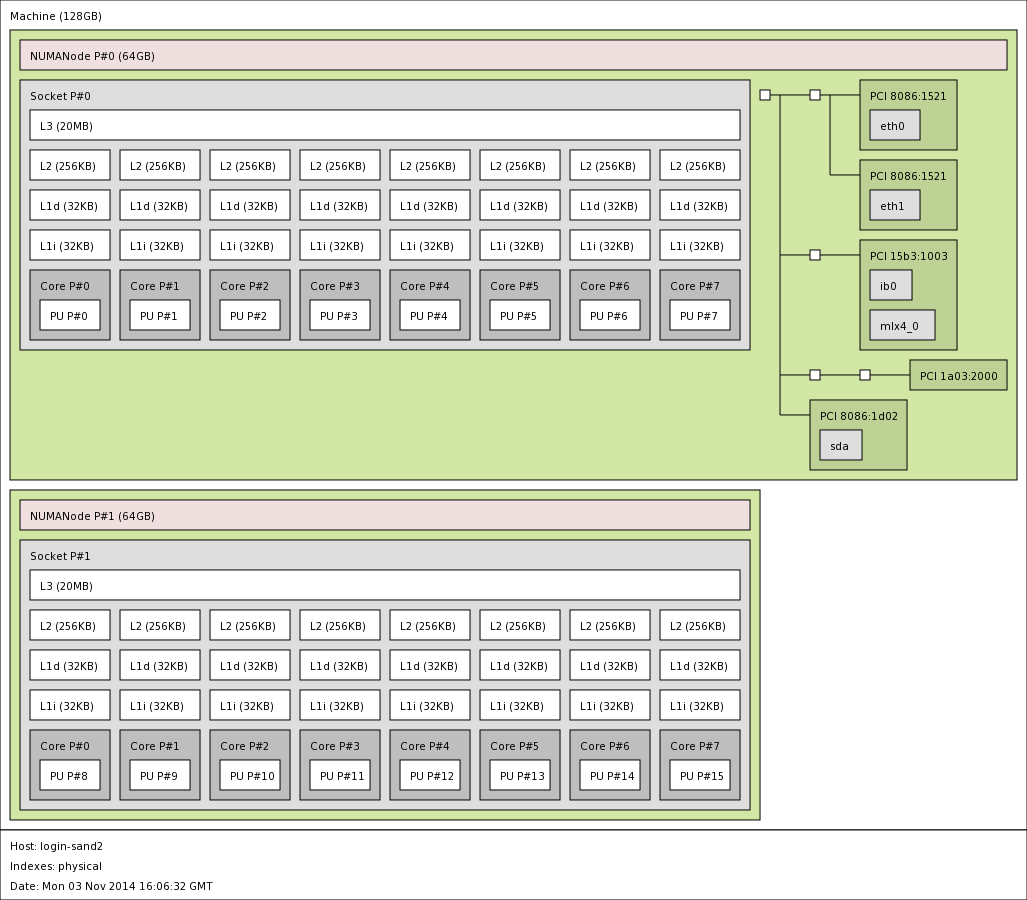
\includegraphics[width=0.8\textwidth]{imgs/lstopo.png}}}
\end{frame}

\subsection{How to Build a Supercomputer pt 1}
\begin{frame}{Advanced: How to Build a Supercomputer}
\only<1,2>{\begin{itemize}
\item{A supercomputer aggregates contemporary CPUs and memory to obtain increased computing power.}
\pause
\item{Usually today these are \alert{clusters}.}
\end{itemize}}
\only<3->{\begin{enumerate}
\item{Take some (multicore) CPUs plus some memory.}
\begin{itemize}
\item<4->{Could be an off-the-shelf server, or something more special.}
\item<5->{A NUMA, shared memory, multiprocessor building block: a \alert{node}.}
\end{itemize}
\end{enumerate}
}
\end{frame}

\subsection{How to Build a Supercomputer pt 2}
\begin{frame}{Advanced: How to Build a Supercomputer}
\begin{tabular}{ll}
\parbox[c]{0.5\textwidth}{\begin{enumerate}
\setcounter{enumi}{1}
\item{Connect the nodes with one or more \alert{networks}. E.g.}
\begin{description}
\item[Gbit Ethernet:]{\alert{100 MB/sec}}
\item[FDR Infiniband:]{\alert{5 GB/sec}}
\end{description}
\pause
\null\par
Faster network is for \alert{inter-CPU communication across nodes}.\par
Slower network is for \alert{management} and \alert{provisioning}.\par
\alert{Storage} may use either.
\end{enumerate}}
&\vbox to 0pt{\vss\vskip 0.25cm\leftline{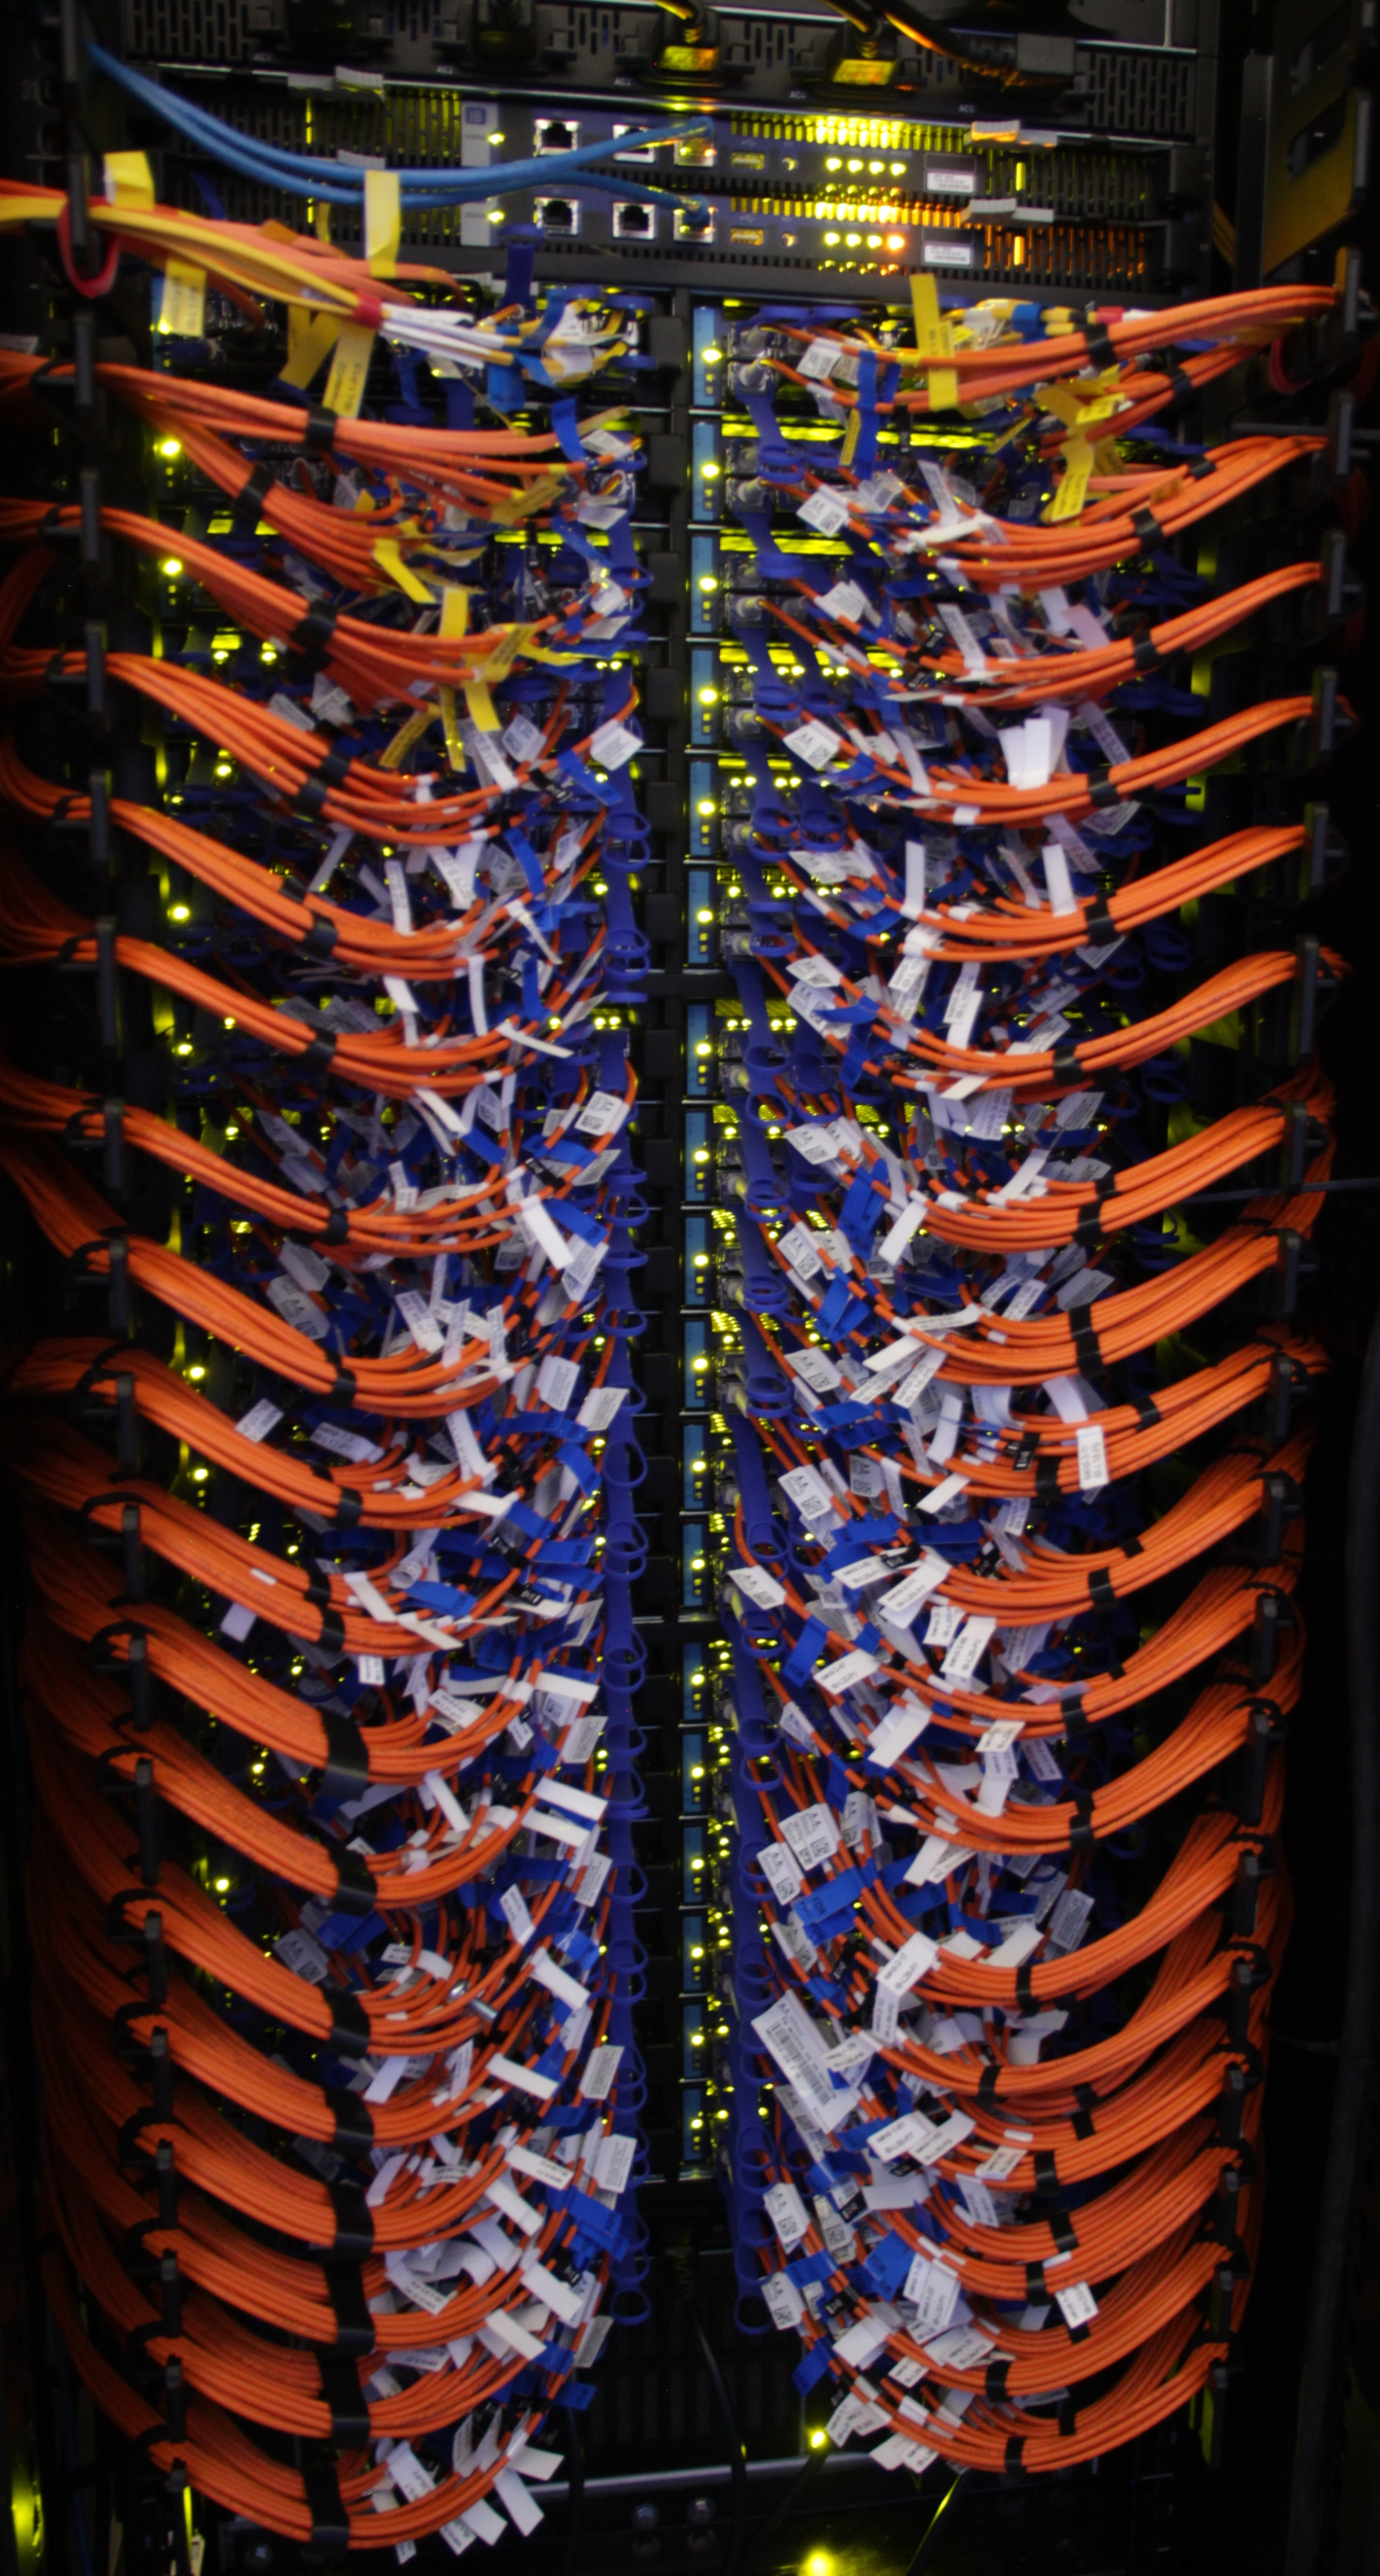
\includegraphics[height=0.85\textheight]{imgs/coreib.jpg}}\vss}\\
\end{tabular}
\end{frame}

\subsection{How to Build a Supercomputer pt 3}
\begin{frame}{Advanced: How to Build a Supercomputer}
\begin{enumerate}
\setcounter{enumi}{2}
\item{Logically bind the nodes}
\begin{itemize}
\item{Clusters consist of distinct nodes (i.e. separate Linux computers)\hfill\\
on common private network(s) and controlled centrally.}
\begin{itemize}
\item[$\ast$]{Private networks allow CPUs in different nodes to communicate.}
\pause
\item[$\ast$]{Clusters are \alert{distributed memory} machines:\hfill\\
\alert{Each process/thread sees only its local node's CPUs and memory (without help).}}
\pause
\item[$\ast$]{\color{red}Each process/thread must fit within a single node's memory.}
\end{itemize}
\pause
\item{More expensive machines logically bind nodes into a single system\hfill\\
{}\qquad i.e. CPUs \alert{and} memory.}
\begin{itemize}
\item[$\ast$]{E.g.\ SGI UV (\alert{COSMOS} system in DAMTP).}
\item[$\ast$]{Private networks allow CPUs to see CPUs and memory in other nodes.}
\pause
\item[$\ast$]{These are \alert{shared memory} machines.}
\item[$\ast$]{Logically a single system - 1 big node - but very non-uniform.}
\item[$\ast$]{A single process can span the entire system.}
\end{itemize}
\end{itemize}
\end{enumerate}
\end{frame}

\section{Programming a Multiprocessor Machine}
\begin{frame}{Advanced HPC: Programming a Multiprocessor Machine}
\only<1-3>{\begin{itemize}
\item{Non-parallel (serial) code}
\begin{itemize}
\item[$\ast$]{\alert{For a single node as for a workstation.}}
\pause
\item[$\ast$]{Typically \alert{run as many copies per node as CPUs}, assuming node memory is sufficent.}
\pause
\item[$\ast$]{\alert{Replicate across multiple nodes.}}
\end{itemize}
\end{itemize}}
\only<4->{\begin{itemize}
\item{Parallel code}
\begin{itemize}
\item<5->[$\ast$]{\alert{Shared memory methods within a node.}\hfill\\
E.g. pthreads, OpenMP.}
\item<6->[$\ast$]{\alert{Distributed memory methods spanning multiple nodes.}\hfill\\
Message Passing Interface (MPI).}
\end{itemize}
\end{itemize}}
\end{frame}

\section*{Summary}

\begin{frame}{Advanced: Summary}
  \begin{itemize}
  \item<1->{\alert{Why have a supercomputer?}}
  \begin{itemize}\item<2->{Big single problems, many problems, Big Data.}\end{itemize}
  \item<3->{Most current supercomputers are \alert{clusters} of separate \alert{nodes}.}
  \item<4->{Each node has \alert{multiple CPUs} and \alert{non-uniform shared memory}.}
  \item<5->{\alert{Parallel} code uses shared memory (\alert{pthreads/OpenMP}) within a node, distributed memory (\alert{MPI}) spanning multiple nodes.}
  \item<6->{\alert{Non-parallel} code uses the memory of one node, but may be copied across many.}
  \end{itemize}
  
\end{frame}

\part{The HPC Service}
\frame{\partpage}

\section{A Brief History of the HPCS}

\begin{frame}{HPCS: A Brief History}
\begin{description}
\item[\alert{Created:}]{1996 (as the HPCF).}
\item[\alert{Mission:}]{Delivery and support of a large HPC resource for use by the University of Cambridge research community.}
\item<2->[\alert{Self-funding:}]{Paying and non-paying service levels.}
\item<2->[\alert{User base:}]{Includes external STFC \& EPSRC plus industrial users.}
\item<3->[\alert{Plus:}]{Dedicated group nodes and research projects.}
%\bigskip
%\item<4->{Absorbed into the UIS in 2014 (part of Research \& Institutional Services).}
\end{description}
\end{frame}

\begin{frame}{The West Cambridge Data Centre}
\centerline{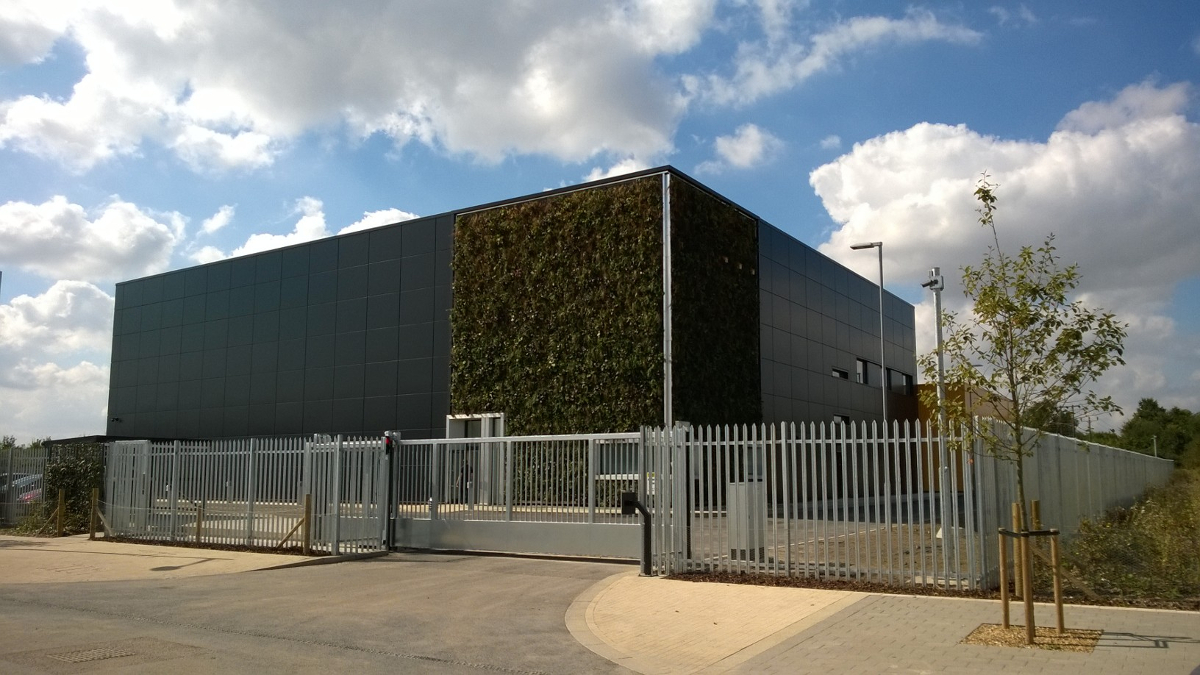
\includegraphics[width=1.05\textwidth]{imgs/WCDC4.jpg}}
\end{frame}

\section{A Brief History of Darwin}
\begin{frame}{HPCS: A Brief History of Darwin}
\begin{description}
\item[1997]{76.8 Gflop/s}
\item[2002]{1.4 Tflop/s}
\item[2006]{18.27 Tflop/s}
\item[2010]{30 Tflop/s}
\item[2012]{183.38 Tflop/s}
\item[2013]{$183.38\,\mbox{CPU}{}+ 239.90\,\mbox{GPU}$ Tflop/s}
\pause
\medskip
\alert{\item[2017]{$\sim1.0\,\mbox{CPU}{}+1.193\,\mbox{GPU}{}+0.508\,\mbox{KNL}{}$ Pflop/s}}
\medskip
\pause
\alert{\item{http://www.top500.org}}
\end{description}
\end{frame}

\begin{frame}<presentation>{Darwin1 (2006--2012)}
\centerline{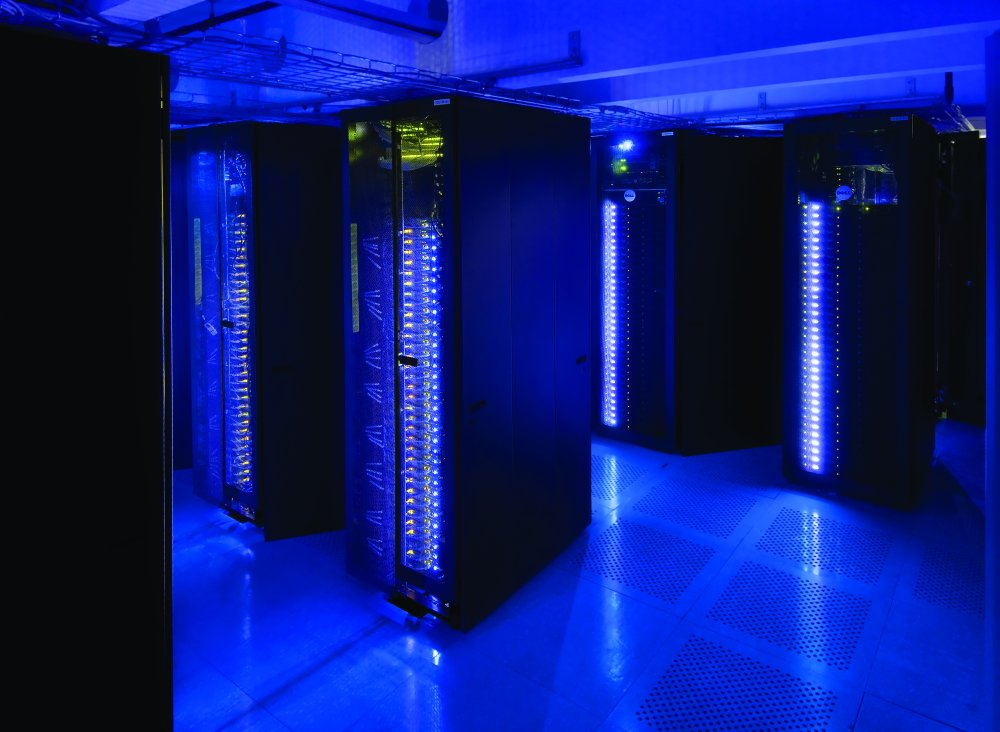
\includegraphics[width=0.875\textwidth]{imgs/darwin.jpg}}%
\smallskip
\end{frame}

\begin{frame}<presentation>{Darwin3 (2012)(b) \& Wilkes (2013)(f)}
\only<1>{\centerline{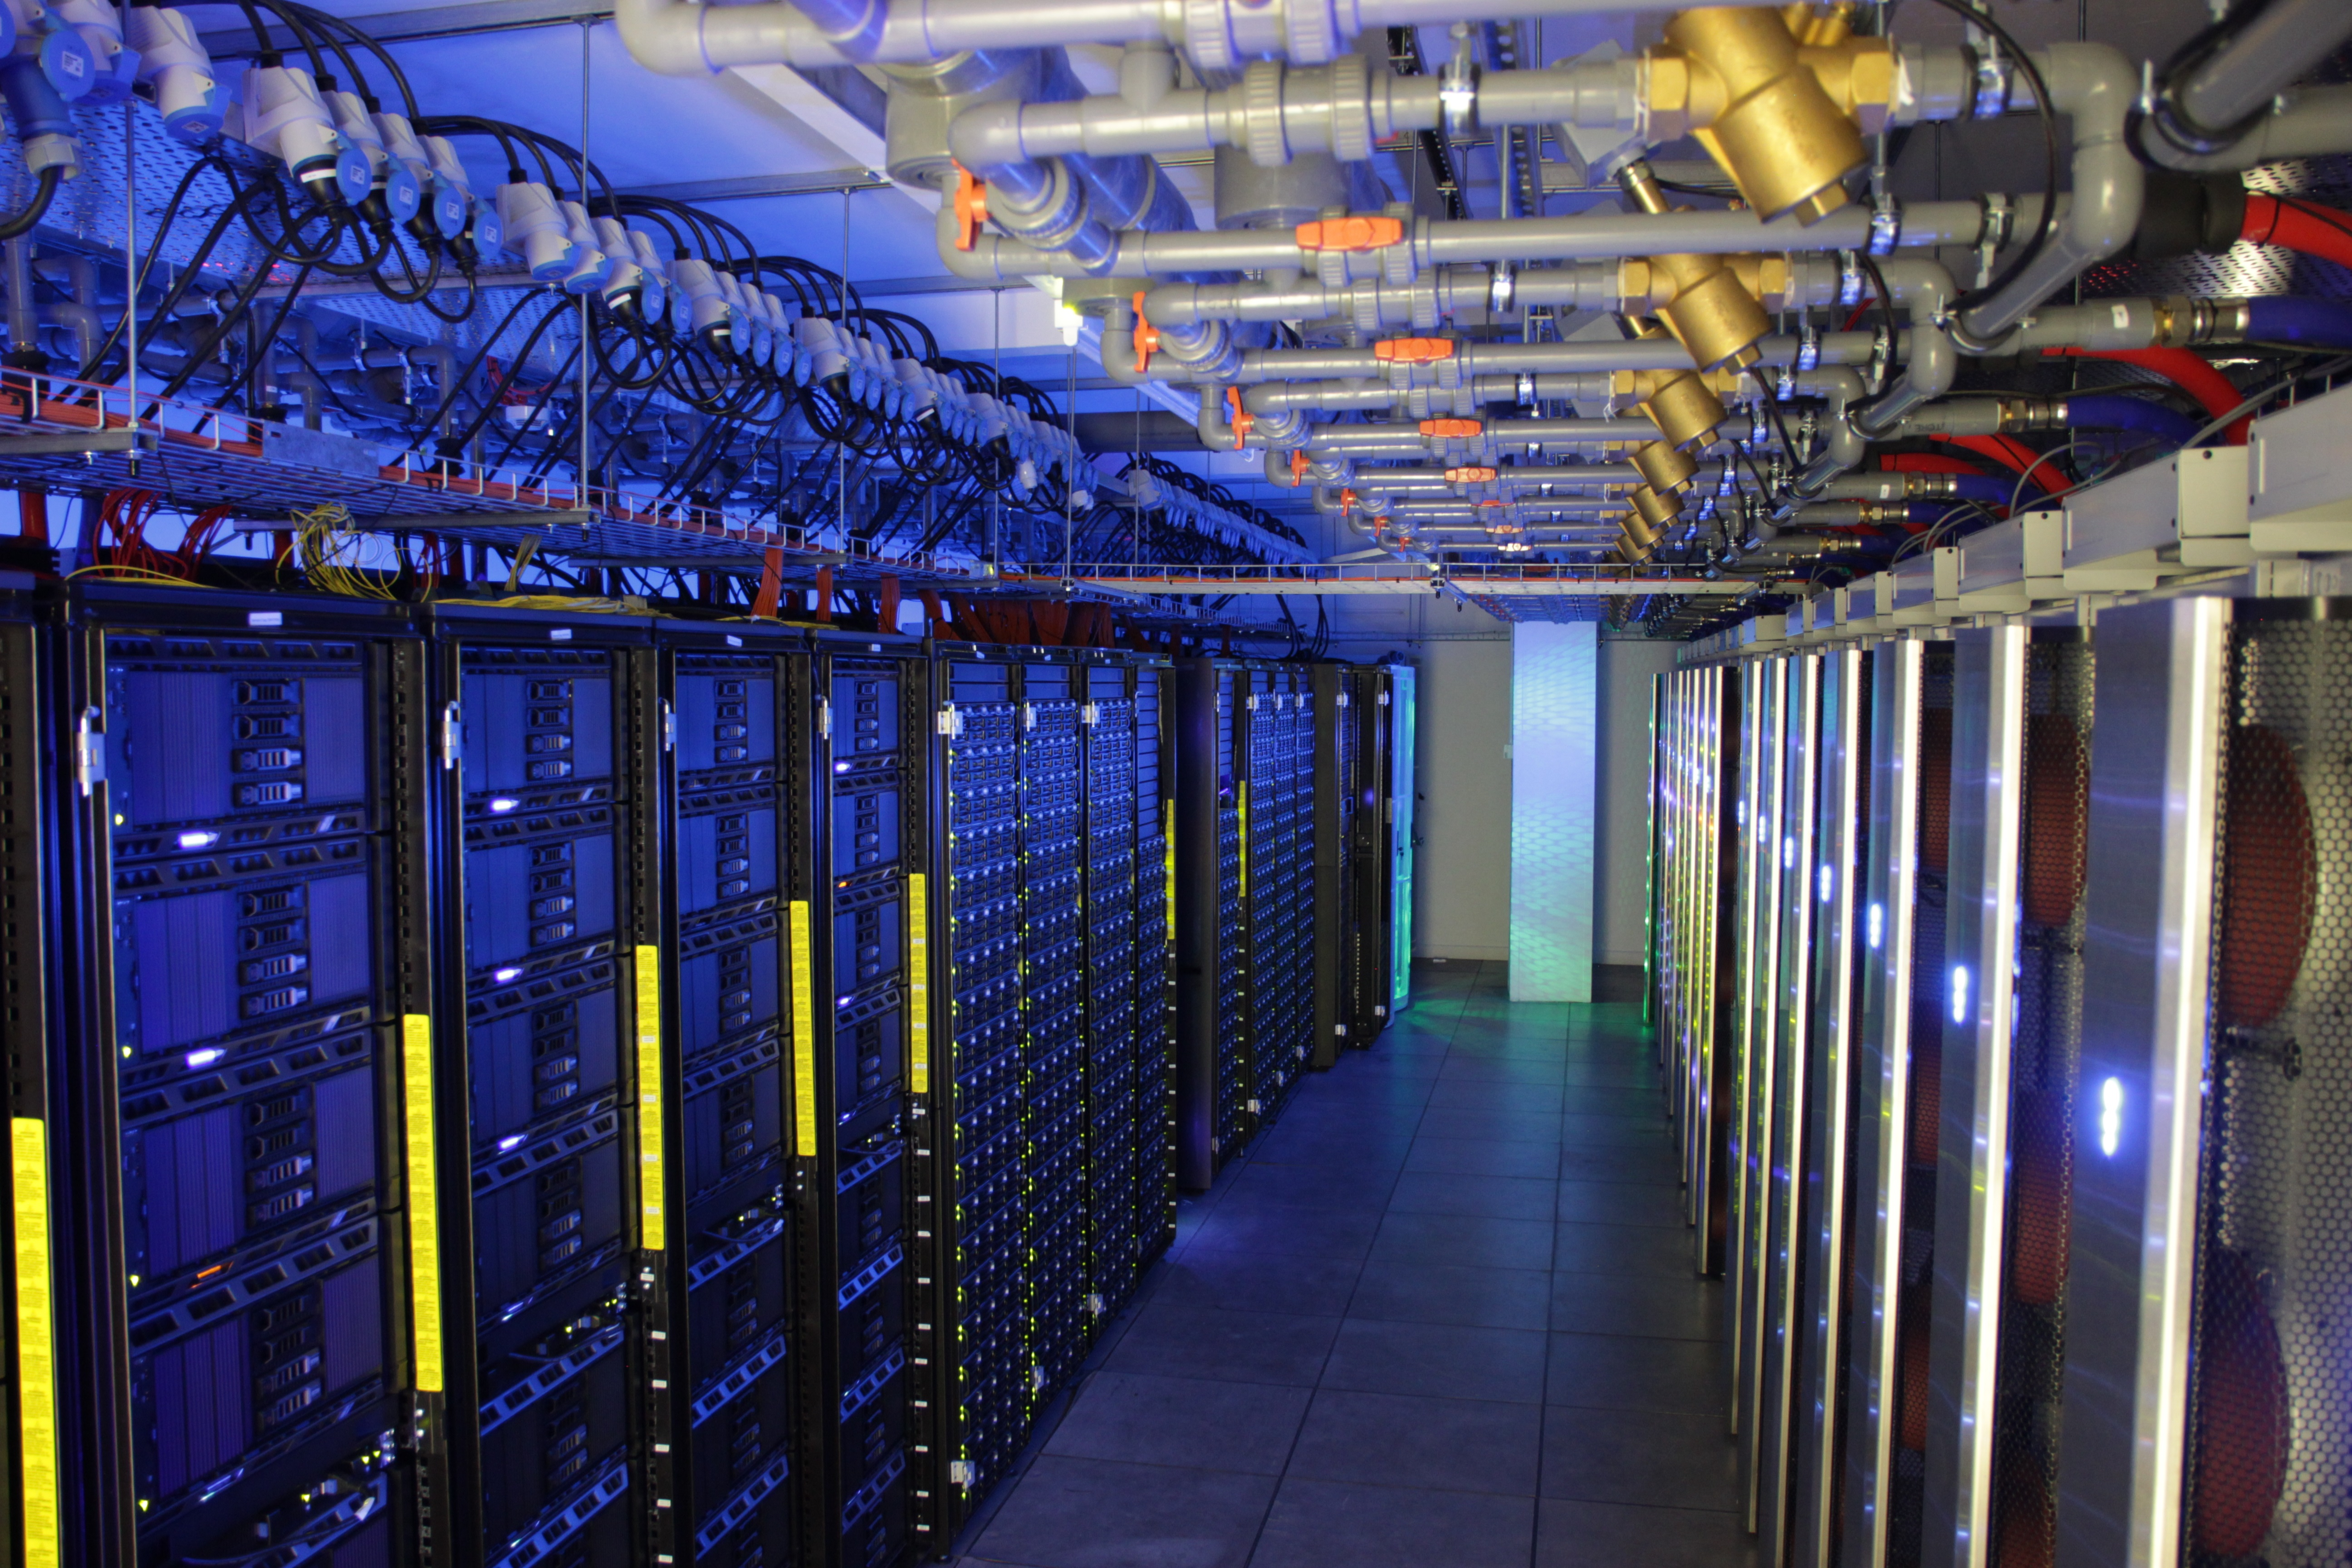
\includegraphics[width=0.95\textwidth]{imgs/MLDC-big.jpg}}}%
%\only<2>{\centerline{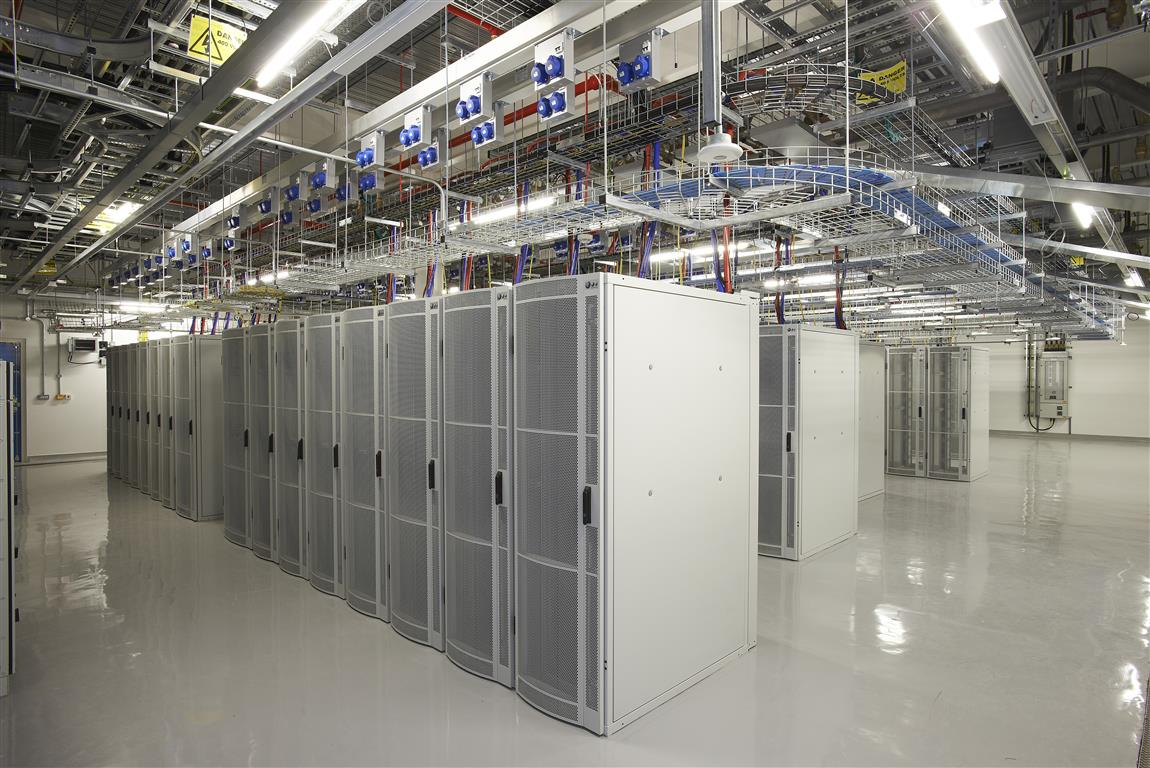
\includegraphics[width=0.95\textwidth]{imgs/WCDC-HPCS.jpg}}}%
\smallskip
\end{frame}

\section{Darwin - an Infiniband CPU Cluster}
\begin{frame}{Darwin: an Infiniband CPU Cluster}
\begin{itemize}
\item{Each compute node:}
\begin{itemize}
\item[$\ast$]{\only<1>{2x8 cores, Intel Sandy Bridge 2.6 GHz.}\only<2->{{\color{red}16 cores}}}
\item[$\ast$]{\only<1>{$64\,\text{GB}$ RAM ($63900\,\text{MB}$ usable).}\only<2->{{\color{red}$63900\,\text{MB}$}}}
\item[$\ast$]{\only<1>{$56\,\text{Gb/sec}$ (4X FDR) Infiniband.}\only<2->{\color{red}$5\,\text{GB/sec}$ Infiniband (for MPI and storage)}}
\end{itemize}
\item{600 compute nodes (300 belong to Cambridge).}
\item{8 login nodes (\alert{login.hpc.cam.ac.uk}).}
\visible<3->{\alert{\item{1 Petaflop upgrade availability October 2017}}}
\end{itemize}
\end{frame}

\section{Wilkes - a Dual-Rail Infiniband GPU Cluster}
\begin{frame}{Wilkes: a Dual-Rail Infiniband GPU Cluster}
\begin{itemize}
\item{Each compute node:}
\begin{itemize}
\item[$\ast$]{\only<1>{$2\times\text{NVIDIA Tesla K20c GPU.}$}\only<2->{\color<2->{red}2 GPUs}}
\item[$\ast$]{\only<1>{2x6 cores, Intel Ivy Bridge 2.6 GHz.}\only<2->{{\color{red}12 cores}}}
\item[$\ast$]{\only<1>{$64\,\text{GB}$ RAM ($63900\,\text{MB}$ usable).}\only<2->{{\color{red}$63900\,\text{MB}$}}}
\item[$\ast$]{\only<1>{$2\times56\,\text{Gb/sec}$ (4X FDR) Infiniband.}\only<2->{\color{red}$2\times5\,\text{GB/sec}$ Infiniband (for MPI and storage)}}
\end{itemize}
\item{128 compute nodes.}
\item{8 login nodes (\alert{login.hpc.cam.ac.uk}).}
\item<3->{Environment shared with Darwin (same filesystems, user environment, scheduler).}
\item<4->{\alert{1 Petaflop upgrade (Wilkes2) early access June 2017}}
\end{itemize}
\end{frame}

\begin{frame}{HPCS Production Cluster Schematic}
\centerline{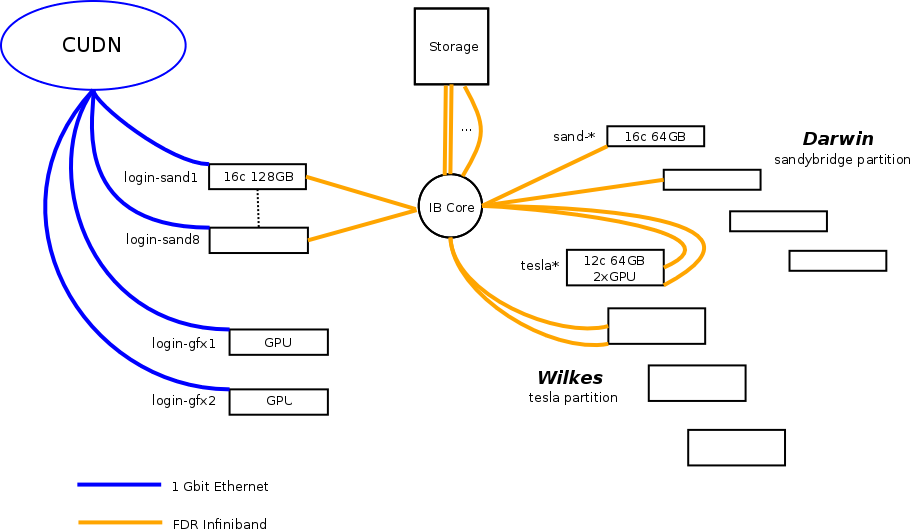
\includegraphics[width=0.95\textwidth]{imgs/cluster.png}}%
\end{frame}

%remote desktop section is normally here

\subsection{Compilers}
\begin{frame}[fragile]{User Environment: Compilers}
\begin{description}
\item[Intel:]{\alert{icc}, \alert{icpc}, \alert{ifort} (recommended)}
\begin{semiverbatim}
\scriptsize
icc -O3 -xHOST -ip code.c -o prog
mpicc -O3 -xHOST -ip mpi_code.c -o mpi_prog
\end{semiverbatim}
\smallskip
\item[GCC:]{\alert{gcc}, \alert{g++}, \alert{gfortran}}
\begin{semiverbatim}
\scriptsize
gcc -O3 -mtune=native code.c -o prog
mpicc -cc=gcc -O3 -mtune=native mpi_code.c -o mpi_prog
\end{semiverbatim}
\smallskip
\item[PGI:]{\alert{pgcc}, \alert{pgCC}, \alert{pgf90}}
\begin{semiverbatim}
\scriptsize
pgcc -O3 -tp=sandybridge code.c -o prog
mpicc -cc=pgcc -O3 -tp=sandybridge mpi_code.c -o mpi_prog
\end{semiverbatim}
\pause
\end{description}
\end{frame}

\section{Modules and Compilers}
\begin{frame}{Exercise 6: Modules and Compilers}
\begin{itemize}
\item{Go to the \alert{exercises} directory of your HPCS training account.}
\visible<2->{\begin{description}
\item[\emph{Hints:}]{\small Firstly you may need to review Exercise 2 in order to reconnect to your HPCS training account. At the HPCS command prompt, change to the exercises directory (\alert{cd $\tilde{}$/exercises}).}
\end{description}}
\item{Try to compile the \alert{hello.c} program using the default \alert{icc} compiler (it will fail because there is a deliberate bug).}
\visible<3->{\begin{description}
\item[\emph{Hints:}]{\small \alert{icc hello.c -o hello}}
\end{description}}
\item{To fix the problem, open the \alert{hello.c} file in the \alert{gedit} editor.}
\visible<4->{\begin{description}
\item[\emph{Hints:}]{\small Launch gedit in the background by doing \alert{gedit\&}. A gedit window should appear. Remove the word \alert{BUG} and save the file.}
\end{description}}
\end{itemize}
\end{frame}

\begin{frame}{Exercise 6: Modules and Compilers (ctd)}
\begin{itemize}
\item{Try again to compile the \alert{hello.c} program using the default \alert{icc} compiler, and run it. You should see \alert{``\emph{node} says: Hello, World!''}.}
\visible<2->{\begin{description}
\item[\emph{Hints:}]{\small \alert{icc hello.c -o hello} then run: \alert{./hello}.}
\end{description}}
\item{Which version of \alert{icc} did you use? Find this out by listing the current modules loaded.}
\visible<3->{\begin{description}
\item[\emph{Hints:}]{\small \alert{module list} --- the Intel compiler modules are named \alert{intel/cce/\emph{version}}.  You can also work out the version directly by finding the location of the binary, e.g.\ doing\hfill\\
\alert{which icc} which should return the path:\hfill\\
\alert{/usr/local/Cluster-Apps/intel/cce/\emph{version}/bin/icc}.}
\end{description}}

\item{Compile and run the \alert{hello.c} program in the exercises directory using a non-default C compiler.}
\visible<4->{\begin{description}
\item[\emph{Hints:}]{\small E.g. load the latest PGI C compiler (\alert{pgcc}) with \alert{module load pgi}. module av will show all possible choices (not all of which are compilers).}
\end{description}}
\end{itemize}
\end{frame}

\section{Job Submission}
\begin{frame}{Using HPC: Job Submission}
\centerline{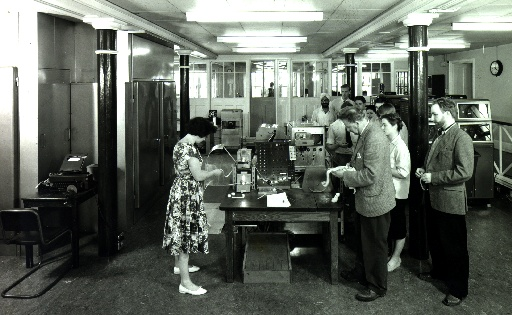
\includegraphics[width=1\textwidth]{imgs/EDSAC_2_1960.jpg}}
\end{frame}
\begin{frame}{Using HPC: Job Submission}
\begin{itemize}
\item{Compute resources are managed by a scheduler:\hfill\\\qquad\alert{SLURM}/PBS/SGE/LSF/\ldots}
\item{Jobs are submitted to the scheduler\hfill\\\qquad --- analogous to submitting jobs to a print queue\hfill\\\qquad --- a file (\emph{submission script}) is copied and queued\hfill\\\qquad \hphantom{---} for processing.}
\end{itemize}
\end{frame}

\begin{frame}{Using HPC: Job Submission}
\begin{itemize}
\item{Jobs are submitted from the \alert{login nodes}\hfill\\\qquad  --- not themselves managed by the scheduler.}
\item{Jobs may be either non-interactive (\alert{batch}) or \alert{interactive}.}
\pause
\item{\alert{Batch} jobs run a shell script on the first of a list of allocated nodes.}
\item{\alert{Interactive} jobs provide a command line on the first of a list of allocated nodes.}
\end{itemize}
\end{frame}

\begin{frame}{Using HPC: Job Submission}
\begin{itemize}
\item{The HPCS has used SLURM since February 2014.}
\item{Jobs may use \alert{part} or \alert{all} of one or more nodes\hfill\\
\qquad --- the owner can specify \mbox{\tt --exclusive} to force exclusive\hfill\\\qquad\hphantom{---} node access (automatic on Wilkes \alert{but may change\hfill\\\qquad\hphantom{---} post-upgrade}).}
\item{Template submission scripts are available under\hfill\\
\qquad \alert{/usr/local/Cluster-Docs/SLURM}.}
\end{itemize}
\end{frame}

\begin{frame}[fragile]{Job Submission: Using SLURM}
\begin{itemize}
\item{Prepare a shell script and submit it to SLURM:}
\begin{semiverbatim}
\scriptsize
[abc123@login]$ sbatch slurm_submission_script
Submitted batch job {\color{red}790299}
\end{semiverbatim}
%\medskip
%\item{PBS (Torque, OpenPBS, PBS Pro)}
%\begin{semiverbatim}
%\scriptsize
%[abc123@login]$ qsub pbs_submission_script
%{\color{red}790299}.master.cluster
%\end{semiverbatim}
\end{itemize}
\end{frame}

\begin{frame}[fragile]{Job Submission: Show Queue}
\begin{itemize}
\item{Submitted job scripts are copied and stored in a queue:}
\begin{semiverbatim}
\tiny
[abc123@login]$ squeue -u abc123
             JOBID PARTITION     NAME     USER  ST       TIME  NODES NODELIST(REASON)
            {\color{red}790299} sandybrid     Test3  abc123 PD       0:00      8 (\only<1>{{\color{blue}Priority}}\only<2>{{\color{green}Resources}}\only<3>{{\color{red}AssocGrpCPUMinsLimit}})
            790290 sandybrid     Test2  abc123  R   27:56:10      8 sand-6-[38-40],sand-7-[27-31]
\end{semiverbatim}
%\medskip
%\item{PBS (Torque, OpenPBS, PBS Pro)}
%\begin{semiverbatim}
%\tiny
%[abc123@login]$ qstat -u abc123
%Job ID               Username    Queue    Jobname          SessID NDS   TSK    Memory Time  S Time
%-------------------- ----------- -------- ---------------- ------ ----- ------ ------ ----- - -----
%790290.master.cl     abc123      tesla    Test2              5519     8     32 248000 36:00 R 27:56
%790281.master.cl     abc123      tesla    Test1             31905     4     16 124000 36:00 C 26:17
%{\color{red}790299}.master.cl     abc123      tesla    Test3               --      8     32 248000 36:00 Q   --
%\end{semiverbatim}
\end{itemize}
\end{frame}

\begin{frame}[fragile]{Job Submission: Monitor Job}
\begin{itemize}
\item{Examine a particular job:}
\begin{semiverbatim}
\scriptsize
[abc123@login]$ scontrol show job={\color{red}790299}
\end{semiverbatim}
%\medskip
%\item{PBS (Torque, OpenPBS, PBS Pro)}
%\begin{semiverbatim}
%\scriptsize
%[abc123@login]$ qstat -f {\color{red}790299}
%\end{semiverbatim}
\end{itemize}
\end{frame}

\begin{frame}[fragile]{Job Submission: Cancel Job}
\begin{itemize}
\item{Cancel a particular job:}
\begin{semiverbatim}
\scriptsize
[abc123@login]$ scancel {\color{red}790299}
\end{semiverbatim}
%\medskip
%\item{PBS (Torque, OpenPBS, PBS Pro)}
%\begin{semiverbatim}
%\scriptsize
%[abc123@login]$ qdel {\color{red}790299}
%\end{semiverbatim}
\end{itemize}
\end{frame}

\begin{frame}[fragile]{Job Submission: Scripts}
\begin{itemize}
\item{SLURM\hfill\\
See \alert{slurm\_submit.darwin}, \alert{slurm\_submit.wilkes}.}
\begin{semiverbatim}
\tiny
#!/bin/bash
#! Name of the job:
{\color<2->{red}#SBATCH} -J darwinjob
#! Which project should be charged:
{\color<2->{red}#SBATCH} -A CHANGEME
#! How many whole nodes should be allocated?
{\color<2->{red}#SBATCH} --nodes=1
#! How many tasks will there be in total? (<= nodes*16)
{\color<2->{red}#SBATCH} --ntasks={\color<3->[rgb]{1,0,0}\only<1-3>{1}\only<4->{16}}
#! How much wallclock time will be required?
{\color<2->{red}#SBATCH} --time=02:00:00
#! Select partition:
{\color<2->{red}#SBATCH} -p sandybridge
...
\end{semiverbatim}
\item<2->{{\color{red}\#SBATCH} lines are \emph{structured comments}\hfill\\
\qquad --- correspond to sbatch command line options.}
\item<3->{\alert{The above job will be given {\color<3->[rgb]{1,0,0}\only<1-3>{1 cpu}\only<4->{16 cpus}} on 1 node for 2 hours (by default there is 1 task per node, and 1 cpu per task).}}
\end{itemize}
\end{frame}

%\begin{frame}[fragile]{Job Submission: Scripts}
%\begin{itemize}
%\item{PBS (Torque, OpenPBS, PBS Pro)}
%\begin{semiverbatim}
%\tiny
%#!/bin/bash 
%#! Name of the job:
%{\color<2->{red}#PBS} -N darwinjob
%#! Which project should be charged:
%{\color<2->{red}#PBS} -A CHANGEME
%#! How many nodes, cores per node, memory and wall-clock time should be allocated?
%{\color<2->{red}#PBS} -l nodes=8:ppn=16,mem=512000mb,walltime=02:00:00
%#! Select queue:
%{\color<2->{red}#PBS} -q sandybridge
%...
%\end{semiverbatim}
%\item<2->{{\color{red}\#PBS} lines are \emph{structured comments}\hfill\\
%\qquad --- correspond to qsub command line options.}
%\end{itemize}
%\end{frame}

\begin{frame}[fragile]{Job Submission: Accounting Commands [HPCS]}
\begin{itemize}
\item{How many core hours available do I have?}
\begin{semiverbatim}
\tiny
mybalance

User            Usage |        Account     Usage | Account Limit Available (CPU hrs)
----------  --------- + -------------- --------- + ------------- ---------
abc123             18 |          STARS       171 |       100,000    {\color{red}99,829}
abc123             18 |      STARS-SL2        35 |       101,000   {\color{red}100,965}
abc123            925 |         BLACKH    10,634 |       166,667   {\color{red}156,033}
\end{semiverbatim}
\smallskip
\item{How many core hours does some other project or user have?}
\begin{semiverbatim}
\tiny
gbalance -p HALOS

User           Usage |   Account     Usage | Account Limit Available (CPU hrs)
---------- --------- + --------- --------- + ------------- ---------

pq345              0 |     HALOS   317,656 |       600,000   {\color{red}282,344}
xyz10         11,880 |     HALOS   317,656 |       600,000   {\color{red}282,344}

(Use -u for user.)
\end{semiverbatim}
\smallskip
\item{List all jobs charged to a project/user between certain times:}
\begin{semiverbatim}
\Tiny
gstatement -p HALOS  -u xyz10 -s "2014-01-01-00:00:00" -e "2014-01-20-00:00:00" 
       JobID      User   Account  JobName  Partition                 End      NCPUS CPUTimeRAW ExitCode      State 
------------ --------- ---------- -------- ---------- ------------------- ---------- ---------- -------- ---------- 
14505            xyz10    halos       help sandybrid+ 2014-01-07T12:59:40         16         32      0:9  COMPLETED 
14506            xyz10    halos       help sandybrid+ 2014-01-07T13:00:11         16         48      2:0     FAILED
...
\end{semiverbatim}
\end{itemize}
\end{frame}


\subsection{Single Node Jobs}
\begin{frame}[fragile]{Job Submission: Single Node Jobs}
\begin{itemize}
\item{Serial jobs requiring large memory, or OpenMP codes.}
\begin{semiverbatim}
\scriptsize
#!/bin/bash
\ldots
#SBATCH --nodes=1
\uncover<2-|handout:2->{{\color{red}#SBATCH --ntasks=1
# Default is 1 task per node}} 
\uncover<3-|handout:2->{{\color{red}#SBATCH --cpus-per-task=\only<3-5|handout:2>{1}\only<6,8-|handout:3,5->{16 # Whole node}\only<7|handout:4>{8  # Half node}
\only<3-5|handout:2>{# Default is 1 cpu (core) per task}}}
\uncover<4-5|handout:2>{{\color{red}#SBATCH --mem=3994
# Memory per node in MB - default is pro rata by cpu number}}
\uncover<5|handout:2>{{\color{red}# Increasing --mem or --cpus-per-task implicitly increases the other}}
\ldots
\uncover<6-|handout:3->{{\color{red}export OMP\_NUM\_THREADS=\only<6|handout:3>{16}\only<7-|handout:4->{8 }  # For OpenMP across \only<6|handout:3>{16}\only<7-|handout:4->{8} cores\only<8-|handout:5->{ (using all memory)}}}
$application \$options
\ldots
\end{semiverbatim}
\end{itemize}
\end{frame}

\subsection{MPI Jobs}
\begin{frame}[fragile]{Job Submission: MPI Jobs}
\begin{itemize}
\item{Parallel job across multiple nodes.}
\begin{semiverbatim}
\scriptsize
#!/bin/bash
\ldots
#SBATCH --nodes={\color{red}4}
#SBATCH --ntasks=\alert{\only<1|handout:1>{64}\only<2-|handout:2->{32}}     # \only<1|handout:1>{i.e.\ {\color[rgb]{0,0.8,0}16}}\only<2-|handout:2->{i.e.\ {\color[rgb]{0,0.8,0} 8}}x{\color{red}4} MPI tasks in total.
\uncover<2-|handout:2->{{\color{red}#SBATCH --cpus-per-task=2}}
\ldots
mpirun\only<2-|handout:2->{ -ppn {\color[rgb]{0,0.8,0}8}} -np \alert{\only<1|handout:1>{64}\only<2-|handout:2->{32}} \$application \$options
\ldots
\end{semiverbatim}
\item<3-|handout:2->{\small SLURM-aware MPI launches remote tasks via SLURM.}
\item<3-|handout:2->{\small The template script uses \$SLURM\_TASKS\_PER\_NODE to set PPN.}
\end{itemize}
\end{frame}

\subsection{Hybrid Jobs}
\begin{frame}[fragile]{Job Submission: Hybrid Jobs}
\begin{itemize}
\item{Parallel jobs using both MPI and OpenMP.}
\begin{semiverbatim}
\scriptsize
#!/bin/bash
\ldots
#SBATCH --nodes={\color{red}4}
#SBATCH --ntasks=\alert{32}     # i.e.\ {\color[rgb]{0,0.8,0} 8}x{\color{red}4} MPI tasks in total.
#SBATCH --cpus-per-task={\color{brown}2}
\ldots
{\color{brown}export OMP\_NUM\_THREADS=2   # i.e.\ 2 threads per MPI task.}
mpirun -ppn {\color[rgb]{0,0.8,0}8} -np \alert{32} \$application \$options
\ldots
\end{semiverbatim}
\item<2->{\small This job uses \alert{64 CPUs} (each MPI task splits into 2 OpenMP threads).}
\end{itemize}
\end{frame}

\subsection{High Throughput Jobs}
\begin{frame}[fragile]{Job Submission: High Throughput Jobs}
\begin{itemize}
\item{Multiple serial jobs across multiple nodes.}
\item{Use \alert{srun} to launch tasks (\alert{job steps}) within a job.}
\begin{semiverbatim}
\scriptsize
#!/bin/bash
\ldots
#SBATCH --nodes=4
\ldots
cd directory\_for\_job1
\alert{srun} {\color<3>{red}--exclusive} {\color<2>{red}-N 1 -n 1} \$application \$options\_for\_job1 > output 2> err {\color<4>{red}&}
cd directory\_for\_job2
\alert{srun} {\color<3>{red}--exclusive} {\color<2>{red}-N 1 -n 1} \$application \$options\_for\_job2 > output 2> err {\color<4>{red}&}
...
cd directory\_for\_job64
\alert{srun} {\color<3>{red}--exclusive} {\color<2>{red}-N 1 -n 1} \$application \$options\_for\_job64 > output 2> err {\color<4>{red}&}
{\color<5>{red}wait}
\end{semiverbatim}
\end{itemize}
\end{frame}

\section{Submitting Jobs}
\begin{frame}{Exercise 7: Submitting Jobs}
\begin{itemize}
\item{Submit a job which will run a copy of your hello program on all cores of 4 of the 24-core nodes which are available for training.}
\visible<2->{\begin{description}
\item[\emph{Hints:}]{\scriptsize\begin{enumerate}
\item{Edit the script \alert{job\_script} in your exercises directory. Set:\hfill\\
\alert{\#SBATCH --nodes=4}\hfill\\
\alert{\#SBATCH --ntasks=96}\hfill\\
\alert{application="./hello"}\hfill\\
In the module section, make sure that the module you used to compile \alert{hello} is also loaded (last).}
\item{Submit the job with \alert{sbatch job\_script}. The jobid is then printed.}
\item{Watch the job in the queue with \alert{squeue}.}
\item{After it has disappeared, open the output file \alert{slurm-jobid.out} in your editor. There should be 24 ``Hello, World!'' messages from 4 different nodes.}
\end{enumerate}%
}
\end{description}}
\end{itemize}
\end{frame}

\begin{frame}{Exercise 7: Submitting Jobs (ctd)}
\begin{itemize}
\item{Experiment with changing the number of nodes and tasks by changing and submitting job\_script (you are limited to 8 nodes in total).}
\end{itemize}
\end{frame}

\subsection{Interactive Jobs}
\begin{frame}[fragile]{Job Submission: Interactive [HPCS]}
\begin{itemize}
\item{Compute nodes are accessible via SSH \alert{while you have a job running on them}.}
\pause
\item{Alternatively, submit an interactive job:}
\begin{semiverbatim}
\alert{sintr -A MYPROJECT -N2 -n16 -t 2:0:0}
\end{semiverbatim}
\medskip
\pause
\item{Within the window (screen session):}
\begin{itemize}
\item[$\ast$]{Launches a shell on the first node (when the job starts).}
\item[$\ast$]{Graphical applications should display correctly.}
\item[$\ast$]{Create new shells with \alert{ctrl-a c}, navigate with \alert{ctrl-a n} and \alert{ctrl-a p}.}
\item[$\ast$]{\alert{ssh} or \alert{srun} can be used to start processes on any nodes in the job.}
\item[$\ast$]{SLURM-aware MPI will do this automatically.}
\end{itemize}
\end{itemize}
\end{frame}


\subsection{Array Jobs}
\begin{frame}[fragile]{Job Submission: Array Jobs}
\begin{itemize}
\item{\color{red}This feature varies between versions.}
\item{\alert{$http://slurm.schedmd.com/job\_array.html$}}
\item{Used for submitting and managing large sets of similar jobs.}
\item{Each job in the array has the same \alert{initial} options.}
\item{SLURM}
\begin{semiverbatim}
\scriptsize
[abc123@login]$ sbatch --array=\only<1,2>{{\color{red}1-7}}\only<2>{{\color{red}:2}}\only<3->{{\color{red}1,3,5,7}} -A STARS-SL2 submission\_script
Submitted batch job {\color[rgb]{0,0.6,0}791609}
\tiny
\uncover<4->{[abc123@login-sand2]$ squeue -u abc123
             JOBID PARTITION     NAME     USER ST       TIME  NODES NODELIST(REASON)
          {\color[rgb]{0,0.6,0}791609}\_{\color{red}1} sandybrid      hpl    abc123  R       0:06      1 sand-6-32
          {\color[rgb]{0,0.6,0}791609}\_{\color{red}3} sandybrid      hpl    abc123  R       0:06      1 sand-6-37
          {\color[rgb]{0,0.6,0}791609}\_{\color{red}5} sandybrid      hpl    abc123  R       0:06      1 sand-6-59
          {\color[rgb]{0,0.6,0}791609}\_{\color{red}7} sandybrid      hpl    abc123  R       0:06      1 sand-7-27
}
\end{semiverbatim}
\uncover<5->{\centerline{{\color[rgb]{0,0.6,0}791609}\_{\color{red}1}, {\color[rgb]{0,0.6,0}791609}\_{\color{red}3}, {\color[rgb]{0,0.6,0}791609}\_{\color{red}5}, {\color[rgb]{0,0.6,0}791609}\_{\color{red}7}}}
\smallskip
\uncover<6->{\centerline{i.e.\ \$\{{\color[rgb]{0,0.6,0}SLURM\_ARRAY\_JOB\_ID}\}\_\$\{{\color{red}SLURM\_ARRAY\_TASK\_ID}\}}}
\smallskip
\uncover<7->{\leftline{\small SLURM\_ARRAY\_JOB\_ID${}={}$SLURM\_JOBID for the first element.}}
\end{itemize}
\end{frame}

\begin{frame}[fragile]{Job Submission: Array Jobs (ctd)}
\begin{itemize}
\item{Updates can be applied to specific array elements using \$\{{\color[rgb]{0,0.6,0}SLURM\_ARRAY\_JOB\_ID}\}\_\$\{{\color{red}SLURM\_ARRAY\_TASK\_ID}\}}
\item{Alternatively operate on the entire array via \$\{{\color[rgb]{0,0.6,0}SLURM\_ARRAY\_JOB\_ID}\}}.
\item{Some commands still require the SLURM\_JOB\_ID (sacct, sreport, sshare, sstat and a few others).}
%\pause
%\item{Exercise 9 - Array Jobs.}
\end{itemize}
\end{frame}

\subsection{Scheduling}
\begin{frame}{Scheduling}
\begin{itemize}
\item{SLURM scheduling is multifactor:}
  \pause
\begin{itemize}
\item{\alert{QoS} --- payer or non-payer?}
  \pause
\item{\alert{Age} --- how long has the job waited?\hfill\\\qquad
  \alert{Don't cancel jobs that seem to wait too long.}}
  \pause
\item{\alert{Fair Share} --- how much recent usage?\hfill\\\qquad
  \alert{Payers with little recent usage receive boost.}}
  \pause
\item{\alert{sprio -j jobid}}
\end{itemize}
\pause
\item{\alert{Backfilling}}
\begin{itemize}
  \item{Promote lower priority jobs into gaps left by higher priority jobs.}
    \item{Demands that the higher priority jobs not be delayed.}
    \item{Relies on reasonably accurate wall time requests for this to work.}
      \item{Jobs of default length will not backfill readily.}
\end{itemize}
\end{itemize}
\end{frame}

\subsection{Wait Times}
\begin{frame}{Wait Times}
  \begin{itemize}
  \item{The cluster is currently very busy and we do not preempt.}
  \item{36 or 12 hour job walltimes are permitted.}
    \pause
  \item{\alert{This sets the timescale at busy times (\emph{without} backfilling).}}
    \pause
  \item{Use backfilling when possible.}
  \item{Short (1 hour or less) jobs have higher throughput (dedicated nodes).}
  \item{Each user can submit \alert{one} very high priority job with \alert{-{}-qos=INTR}.}
    \pause
    \item{We are upgrading significantly in 2017!}
\end{itemize}
\end{frame}

\subsection{Checkpointing}
\begin{frame}{Checkpointing}
  \begin{itemize}
  \item{Insurance against failures during long jobs.}
  \item{Restart from checkpoints to work around finite job length.}
    \pause
  \item{Application native methods are best. Failing that $\ldots$}
    \pause
  \item{Darwin \& Wilkes nodes currently provide Berkeley Lab Checkpoint/Restart (BLCR)\hfill\\
  \qquad\alert{cr\_run, cr\_checkpoint, cr\_restart}}
    \item{\alert{sbatch -{}-checkpoint=minutes}}
    \item{\alert{scontrol checkpoint restart jobid}}
  \end{itemize}
\end{frame}

\subsection{Scheduling Top Tips}
\begin{frame}{Job Submission: Scheduling Top Dos \& Don'ts}
\begin{itemize}
\item{\textbf{Do \ldots}}
\begin{itemize}
\item{Give reasonably accurate wall times (allows \alert{backfilling}).}
\item{Check your balance occasionally (\alert{mybalance}).}
\item{Test on a small scale first.}
\item{Implement \alert{checkpointing} if possible (reduces resource wastage).}
\end{itemize}
\medskip
\item{\textbf{Don't \ldots}}
\begin{itemize}
\item{Request more than you need\hfill\\
\qquad --- you will wait longer and use more credits.}
\item{Cancel jobs unnecessarily\hfill\\
\qquad ---  priority increases over time.}
\end{itemize}
\end{itemize}
\end{frame}
\end{document}